\chapter{Unsupervised Learning}
\section{Dimensional Reduction and Data Visualization}
\label{sec:dimRed}
In this section, we will begin our foray into unsupervised learning by way of data visualization. Data visualization methods are important for modelling as they can be used to identify correlated or redundant features along with irrelevant features (noise) from raw or processed data. For data involving a relatively small number of features, studying pair-wise correlations (i.e. pairwise scatter plots of all features) may suffice in performing a complete analysis. This rapidly becomes impractical for datasets involving a large number of measured features (such as images). \begin{mybox}{Dimensional Reduction}
	Thus, in practice, we often have to perform \emph{dimensional reduction}, namely, project or embed the data onto a lower dimensional space, which we refer to as the \emph{latent} space.\\
	A recurrent objective of dim. red. techniques is to preserve the relative pairwise distances (or defined similarities) between data points from the original space to the latent space.
\end{mybox}
Part of the complication of dim. red. lies in the fact that low-dimensional representations of high-dimensional data necessarily incurs information loss.

\subsection{Some of the challenges of high-dimensional data}
\label{subsec:dimRedChallengesData}
\subsubsection{High-dimensional data lives near the edge of sample space}
Like one sees in statistical physics, for high-dimensional data, approximately all of the datapoints are contained only in the surface of the $D$-dimensional sphere/cube/... describing it.

\subsubsection{Real-world data vs. uniform distribution}
Fortunately, real-world data is not random or uniformly distributed.\\
In facet, real data usually lives in a much lower dimensional space than the original space in which the features are being measured. This is sometimes referred to as the \emph{blessing of non-uniformity} (in opposition to the curse of dimensionality \ref{subsubsec:performanceevalCurseDimensionality}). 
\begin{example}
	For weakly interacting particles in stat. phys., one can describe them via thermodynamic variables containing the macroscopic dynamics without having to specify the high-dimensional $N\propto 10^{23}$ amount of d.o.f. of the respective phase space dynamics of every particle in the ensemble.
\end{example}

\subsubsection{Intrinsic dimensionality and the crowding problem}
\begin{mybox}{Intrinsic dimensionality of the data}
	Qualitatively, this refers to the minimum number of dimensions (parameters) required to capture the signal in the data (to parametrize the data).  For example, if a data set is described by a sphere, then you need three parameters ($r,\vartheta,\varphi$), i.e. an intrinsic dimensionality of $3$, to parametrize the sphere $S^2 \subset \mR^3$.
\end{mybox}
\begin{mybox}{Crowding problem}
	Attempting to represent data in a space of dimensionality lower than its intrinsic dimensionality can lead to a \emph{crowding problem}. In short, because we are attempting to satisfy too many constraints (e.g. preserve all relative distances of the original space), this results in a trivial solution for the latent space where all mapped data points collapse to the centre of the map. In our example, if you collapse the sphere into two-dimensions, i.e. the circle with variable radius, the two hemispheres would be projected non-bijectively onto the circle, i.e. $\vartheta\in [0,\pi)\mapsto \vartheta=const$. Thus, you would lose a lot of information via the embedding in $\mR^2$.
\end{mybox}
To alleviate this, one needs to weaken the constraints imposed on the visualization scheme. Powerful methods such as t-distributed stochastic embedding (t-SNE) and uniform manifold approximation and projection (UMAP) have been devised to circumvent this issue in various ways.


\subsection{Principal component analysis (PCA)}
\label{subsec:dimRedPCA}
\begin{mybox}{PCA}
A ubiquitous method for dimensional reduction, data visualization and analysis is \emph{Principal Component Analysis} (PCA). The goal of PCA is to perform an orthogonal transformation of the data in order to find high-variance directions. PCA is inspired by the observation that in many cases, the relevant information in a signal is contained in the directions with largest variance. This can be seen as ’fitting’ an ellipse to the data with the major axis corresponding to the first principal component (direction of largest variance).
\end{mybox}
Such PCA-based projections often capture a lot of the large scale structure of many datasets. Even without prior physical knowledge, one can extract relevant order parameters using a simple PCA-based projection.
\subsubsection{The theory}
\label{subsubsec:dimRedPCAtheory}
Consider $N$ data points, $\{\mx_1,\dots,\mx_N\}$ that live in a $p$-dimensional feature space $\mx_i \in \mR^p$. Denote the $N\times p$ design matrix as $\mX = [\mx_1,\dots,\mx_N]^T$ whose rows are the data points and columns correspond to different features, compare \ref{subsec:recipeML}. The $p\times p$ (symmetric) covariance matrix is therefore 
\be 
\label{eq:dimRedPCAcovMatrix}
\mS(\mX) = \frac{1}{N-1} \mX^T \mX.
\ee 
notice that the $j$-th diagonal entry of $\mS(\mX)$ corresponds to the variance of the $j$-th feature and $\mS(\mX)_{ij}$ measures the covariance (i.e. connect correlation in the language of physics) between feature $i$ and feature $j$.\\
Via singular value decomposition (SVD), one finds
\be 
\mS(\mX) = \mathbf{V} \left(\frac{\mathbf{S}^2}{N-1}\right) \mathbf{V}^T \equiv \mathbf{V}\mathbf{Λ} \mathbf{V}^T,
\ee 
where $\mathbf{V}$ contains (as its columns) the right singular vectors of $\mX$, and $\mathbf{Λ}$ is a diagonal matrix with eigenvalues $\lambda_i =s^2_i/(N-1)$ ($s_i$ are the singular values) in the decreasing order along the diagonal (i.e. eigendecomposition). It is clear that the right singular vectors of $\mX$ (i.e. the columns of $\mathbf{V}$) are principal directions of $\mS(\mX)$, and the singular values of $\mX$ are related to the eigenvalues of the covariance matrix $\Sigma(\mX)$ via $\lambda_i$. To reduce the dimensionality of data from $p$ to $\tilde{p}<p$, we first construct the $p\times \tilde{p}$ projection matrix $\mathbf{V}_{\tilde{p}}$ by selecting the singular components with the $\tilde{p}$ largest singular values. The projection of the data from $p$ to $\tilde{p}$ is simply $\tilde{\mathbf{Y}}=\mX \mathbf{V}_{\tilde{p}}$. \\
The singular vector with the largest singular value (i.e. the largest variance) is referred to as the first principal component; the singular vector with the second largest singular value as the second principal component, and so on. An important quantity is the ratio $\lambda_i/\sum_{i=1}^p \lambda_i$ which is referred as the \emph{percentage of the explained variance contained in a principal component}.\\
It is common in data visualization to present the data projected on the first few principal components. This is valid as long as a large part of the variance is explained in those components. Low values of explained variance may imply that the intrinsic dimensionality of the data is high or simply that it cannot be captured by a linear representation.

\subsection{Multidimensional scaling}
\label{subsec:dimRedMDS}
\begin{mybox}{MDS}
	Multidimensional scaling (MDS) is a non-linear dimensional reduction technique which preserves the pairwise distance or dissimilarity $d_{ij}$ between data points. There are two types of MDS, metric and non-metric.
\end{mybox}
\subsubsection{Metric MDS}
In metric MDS, the distance is computed under a pre-defined metric and the latent coordinates $\tilde{\mathbf{Y}}$ are obtained by minimizing the difference between the distance measured in the original space ($d_{ij}(\mx)$) and that in the latent space ($d_{ij}(\mathbf{Y})$):
\be 
\label{eq:dimRedMDS}
\tilde{\mathbf{Y}} = \arg \min_{\mathbf{Y}} \sum_{i<j} w_{ij} \abs{d_{ij} (\mX)-d_{ij}(\mathbf{Y})},
\ee 
where $w_{ij}\geq 0$ are weight values. The weight matrix $w_{ij}$ is a set of free parameters that specify the level of confidence (or precision) in the value of $d_{ij}(\mX)$. If Euclidean metric is used, MDS gives the same result as PCA and is usually referred to as classical scaling. Thus MDS is often considered as a generalization of PCA.

\subsubsection{Non-metric MDS}
In non-metric MDS, $d_{ij}$ can be any distance matrix. The objective function is then to preserve the ordination in the data, i.e. if $d_{12}(\mX) < d_{13}(\mX)$  in the original space, then in the latent space we should have $d_{12}(\mathbf{Y})< d_{13}(\mathbf{Y})$.

\subsubsection{General comment}
Both MDS and PCA can be implemented using standard Python packages such as Scikit. They are often among the first data visualization techniques one resorts to.

\subsection{t-SNE}
\label{subsec:dimRedTSNE}
It is often desirable to preserve local structures in high-dimensional datasets. However, when dealing with datasets having clusters delimitated by complicated surfaces or datasets with a large number of clusters, preserving local structures becomes difficult using linear techniques such as PCA\footnote{Non-linear techniques such as non-classical MDS, self-organizing map, Isomap and Locally Linear Embedding preserve local structures but fail to capture structures at the larger scale such as the clusters in which the data is organized.}.
\marginpar{Non-parametric here means that it does not explicitly parametrize feature extraction required to compute the embedding coordinates. Thus it cannot be applied to find the coordinate of new data points.}
\begin{mybox}{t-SNE}
	Recently, $t$-stochastic neighbour embedding ($t$-SNE) has emerged as one of the go-to methods for visualizing high-dimensional data. $t$-SNE is a non-parametric method that constructs non-linear embeddings. Each high-dimensional training point is mapped to low-dimensional embedding coordinates, which are optimized in a way to preserve the local structure in the data.
\end{mybox}
\subsubsection{The theory}
The idea of stochastic neighbour embedding is to associate a probability distribution to the neighbourhood of each data (note $x\in \mR^p$, $p$ is the number of features):
\be 
p_{i|j} = \frac{\exp(-\norm{x_i-x_j}^2/2 \sigma^2_i)}{\sum_{k\neq i} \exp(-\norm{x_i-x_k}^2/2 \sigma^2_i)},
\ee 
where $p_{i|j }$ can be interpreted as the likelihood that $x_j$ is $x_i$'s neighbour (thus we take $p_{i|i}=0$). $\sigma_i$ are free bandwidth parameters that are usually determined by fixing the local entropy $H(p_i)$ of each data point:
\be 
H(p_i) \equiv -\sum_j p_{j|i}\log_2 p_{j|i}.
\ee 
The local entropy is then set to equal a constant across \emph{all data points} $\Sigma = 2^{H(p_i)}$, where $\Sigma$ is called the \emph{perplexity}. The perplexity constraint determines $\sigma_i \forall i$ and implies that points in regions of high-density will have smaller $\sigma_i$.\\
\\
Using Gaussian likelihoods in $p_{i|j}$ implies that only points that are nearby $x_i$ contribute to its probability distribution. This ensures that the similarity for nearby points is well represented but neglects the contributions of points far away. To alleviate this, we define a symmetrized distribution $p_{ij} \equiv (p_{i|j}+p_{j|i})/(2N)$. This \emph{guarantees} that $\sum_j p_{ij} >1/(2N)$ for all data points $x_i$, resulting in each data point $x_i$ making a significant contribution to the cost function to be defined below.
\begin{mybox}{tSNE}
	$t$-SNE constructs a \emph{similar} probability distribution $q_{ij}$ in a low dimensional latent space (with coordinates $Y=\{y_i\}, y_i \in \mR^{p^\prime}$, where $p^\prime <p$ is the dimension of the latent space):
	\be 
	\label{eq:dimRedTSNEprobdistr}
	q_{ij} = \frac{(1+\norm{y_i-y_j}^2)^{-1}}{\sum_{k\neq i} (1+\norm{y_i-y_k}^2)^{-1}}.
	\ee 
	The crucial point to note is that $q_{ij}$ is chosen to be a longtail distribution. This preserves short distance information (relative neighbourhoods) while strongly repelling two points that are far apart in the original space.\\
	In order to find the latent space coordinates $y_i$, $t$-SNE minimizes the Kullback-Leibler divergence between $q_{ij}$ and $p_{ij}$:
	\be 
	\label{eq:dimRedTSNECostfct}
	\mC(Y) = D_{KL} (p||q) \equiv \sum_{ij} p_{ij} \log\left(\frac{p_{ij}}{q_{ij}}\right).
	\ee 
	This minimization is done via GD (see \ref{sec:gd}).
\end{mybox}
Computing the gradient of \ref{eq:dimRedTSNECostfct}, we can see what the embedding cost-function $\mC$ is capturing
\begin{align}
	\label{eq:dimRedTSNEForce}
	\partial_{y_i} \mC&=\sum_{j\neq i} 4 p_{ij} q_{ij} Z_i(y_i-y_j) - \sum_{j\neq i} 4 q^2_{ij} Z_i(y_i-y_j)\nonumber \\
	&= F_{\text{attractive,}i} -F_{\text{repulsive,}i},
\end{align}
where $Z_i=1/(\sum_{k\neq i} (1+\norm{y_k-y_i}^2)^{-1})$. Notice that $F_{\text{attractive,}i}$ induces a significant attractive force only between points that are nearby point $i$ in the \emph{original space} since it involves the $p_{ij}$ term. Finding the embedding coordinates $y_i$ is thus equivalent to finding the equilibrium configuration of particles interacting through forces, compare \ref{eq:dimRedTSNEForce}.\\
\\
The $t$-SNE visualization cleanly separates all the clusters while certain clusters blend together in PCA for example. This is a direct consequence of the fact that $t$-SNE keeps nearby points close together while repelling points that are far apart, compare \ref{eq:dimRedTSNEForce}.

\subsubsection{Important properties of $t$-SNE}
\begin{enumerate}
\item $t$-SNE can rotate data:\\
The KL divergence is invariant under rotations in the latent space, i.e. $t$-SNE plots that are rotations of each other should be considered equivalent.
\item $t$-SNE results are stochastic.\\
In applying GD, the solution of different $t$-SNE runs depends on the initial seed and results in different outcomes.
\item \emph{$t$-SNE generally preserves short distance information}.\\
As a rule of thumb, one should expect that nearby points on the $t$-SNE map are also closeby in the original space, i.e. $t$-SNE tends to preserve ordination (but not actual distances).
\item \emph{Scales are deformed in $t$-SNE}.\\
Since a scale-free distribution is used in the latent space, one should not put too much emphasis on the meaning of the size of any clusters observed in the latent space.
\item \emph{$t$-SNE is computationally intensive}:\\
$\mO(N^2)$.
\end{enumerate}





\section{Clustering}
\label{sec:cluster}
This section is also concerned with unsupervised learning methods.\\
Unsupervised learning is concerned with discovering structure in unlabelled data (for instance learning local structures for data visualization \ref{sec:dimRed}). The lack of labels make unsupervised learning much more difficult and subtle than its supervised counterpart. What is somewhat surprising is that even without labels it is still possible to uncover and exploit the hidden structure in the data. Perhaps, the simplest example of unsupervised learning is clustering.
\begin{mybox}{Clustering}
 The aim of clustering is to group unlabelled data into clusters according to some similarity or distance measure. Informally, a cluster is thought of as a set of points sharing some pattern or structure.\\
 Clustering finds many applications throughout data mining, data compression and signal processing. Clustering can be used to identify coarse features or high level structures in an unlabelled dataset.
\end{mybox}
The field of clustering is vast and there exists a flurry of clustering methods suited for different purposes. Some common considerations one has to take into account when choosing a particular method is the distribution of the clusters (overlapping/noisy clusters vs. well-separated clusters), the geometry of the data (flat vs. non-flat), the cluster size distribution (multiple sizes vs. uniform sizes), the dimensionality of the data (low vs. high dimensional) and the computational efficiency of the desired method (small vs. large dataset).


\subsection{Practical clustering methods}
\label{subsec:clusterPractical}
Throughout this section we focus on the Euclidean distance as a similarity measure.

\subsubsection{$K$-means}
\label{subsubsec:clusterPracticalKmeans}

Consider a set of $N$ \emph{unlabelled} observations $\{\mx_n\}^N_{n=1}$ where $\mx_n\in \mR^p$ and where $p$ is the number of features. Also consider a set of $K$ cluster centres called the cluster \emph{means}: $\{\mathbf{μ}_k\}^K_{k=1}$, with $\mathbf{μ}_k\in \mR^p$, which we'll compute ’empirically’ in the clustering procedure. The cluster means can be thought of as the representatives of each cluster, to which data points are assigned. 
\begin{mybox}{$K$-means set-up}
	$K$-means clustering can be formulated as follows: given a fixed integer $K$, find the cluster means $\{\mathbf{μ}\}$ and the data point assignments in order to minimize the following objective function
	\be
	\label{eq:clusterPracticalKmeansCostfct}
	\mC(\{x,\mathbf{μ}\}) = \sum_{k=1}^K \sum_{n=1}^N r_{nk} ( \mx_n - \mathbf{μ}_k)^2,
	\ee
	where $r_{nk} \in \{0,1\}$ is a binary variable called the \emph{assignment}. The assignment $r_{nk}$ is $1$ if $x_n$ is assigned to cluster $k$ and $0$ otherwise. Notice that $\sum_k r_{nk}=1 \forall n$ and $\sum_n r_{nk}\equiv N_k$, where $N_k$ is the number of points assigned to cluster $k$. The minimization of this objective function can be understood as trying to find the best cluster means such that the variance within each cluster is minimized.
\end{mybox}
In physical terms, $\mC$ is equivalent to the sum of the moments of inertia of every cluster. The cluster means $\mathbf{μ}_k$ correspond to the centres of mass of their respective cluster.
\begin{mybox}{$K$-means algorithm}
	The $K$-means algorithm alternates between two steps:
	\begin{enumerate}
		\item \emph{Expectation}: Given a set of assignments $\{r_{nk}\}$, minimize $\mC$ w.r.t. $\mathbf{μ}_k$. Taking a simple derivative and setting it to zero yields the following update rule:
		\be 
		\mathbf{μ}_k = \frac{1}{N_k} \sum_n r_{nk} \mx_n.
		\ee 
		\item \emph{Maximization}: Given a set of cluster means $\{\mathbf{μ}_k\}$, find the assignments $\{r_{nk} \}$ which minimize $\mC$. Clearly, this is achieved by assigning each data point to their nearest cluster-mean:
		\be
		r_{nk} = \left\{ \begin{array}{ll}
		1 & \text{if } k=\arg \min_{k^\prime} (\mx_n-\mathbf{μ}_{k^\prime})^2 \\
		0& \text{otherwise}.
		\end{array}\right\}
		\ee 
	\end{enumerate}
Practically, the algorithm should terminate when the change in the objective function from one iteration to another becomes smaller than a pre-specified threshold.
\end{mybox}
A nice property of the $K$-means algorithm is that it is guaranteed to converge.\footnote{To see this, one can verify explicitly (by taking second-order derivatives) that the expectation and assignment step respectively always decrease $\mC$. Thus, since $\mC$ is bounded from below, the two-step iteration of $K$-means \emph{always} converges to a local maximum of $\mC$. Since $\mC$ is generally a non-convex function, in practice one usually needs to run the algorithm with different initial random cluster centre initializations and post-select the best local minimum.} The complexity is $\mO(KN)$ per iteration and is thus scalable to very large datasets.\\
A common drawback of $K$-means is the following:\\
If the true clusters have very different variances (spreads), $K$-means can lead to spurious results since the underlying assumption is that the latent model has uniform variances.\\
\\
We can measure the performance of $K$-means by thinking about the distortion- the square distance of each point from the centroid defining the cluster. This is the objective function that K-means tries to optimize.

\subsubsection{Hierarchical clustering: Agglomerative methods}
\label{subsubsec:clusterPracticalHierarchical}
Agglomerative clustering is a bottom up approach that starts from small initial clusters which are then progressively merged to form larger clusters.
\begin{figure}[h!]
	\centering
	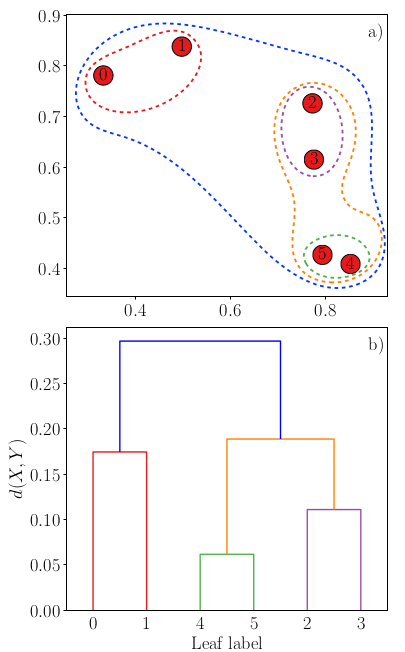
\includegraphics[width=0.4\linewidth]{gfx/HierarchicalCLustering}
	\caption{\itshape The merging process generates a hierarchy of clusters that can be visualized in the form of a dendrogram.}
	\label{fig:hierarchicalclustering}
\end{figure}
This hierarchy \ref{fig:hierarchicalclustering} can be useful to analyze the relation between clusters and the subcomponents of individual clusters. Agglomerative methods are usually specified by defining a distance measure between clusters. Different choices of distance result in different clustering algorithms. At each step, the two clusters that are the closest w.r.t. the distance measure are merged until a single cluster is left.

\begin{mybox}{Agglomerative clustering algorithm}
	\begin{enumerate}
		\item Initialize each point to its own cluster.
		\item Given a set of $K$ clusters $X_1,X_2,\dots,X_K$, merge clusters until one cluster is left ($K=1$):
		\begin{enumerate}
			\item Find the closest pair of clusters $(X_i,X_j)$:
			\bse 
			(i,j)=\arg \min_{i^\prime,j^\prime} d(X_{i^\prime},X_{j^\prime} )
			\ese 
			\item Merge the pair. Update. $K\leftarrow K-1$.
		\end{enumerate}
	\end{enumerate}
\end{mybox}
The most popular distances used in agglomerative methods, often called \emph{linkage methods}
\begin{enumerate}
	\item Single-linkage: the distance between clusters $i$ and $j$ is defined as the minimum distance between two elements of the different clusters
\be
\label{eq:ClusterPracticalHierarchicalSinglelinkage}
d(X_i,X_j) = \min_{\mx_i \in X_i,\mx_j \in X_j} \norm{\mx_i-\mx_j}_2. 
\ee 
\item Complete linkage: the distance between clusters $i$ and $j$ is defined as the maximum distance between two elements of the different clusters
\be 
\label{eq:ClusterPracticalHierarchicalCompleteLinkage}
d(X_i,X_j) = \max_{\mx_i \in X_i,\mx_j\in X_j} \norm{\mx_i-\mx_j}_2.
\ee 
\item Average linkage: average distance between points of different clusters
\be 
\label{eq:ClusterPracticalHierarchicalAverageLinkage}
d(X_i,X_j) = \frac{1}{\abs{X_i}\cdot \abs{X_j}} \sum_{\mx_i \in X_i,\mx_j\in X_j} \norm{\mx_i-\mx_j}_2.
\ee 
\item Ward's linkage: This distance measure is analogous to the $K$-means method as it seeks to minimize the total inertia. The distance measure is the ’error squared’ before and after merging which simplifies to
\be 
\label{eq:ClusterPracticalHierarchicalWardsLinkage}
d(X_i,X_j) = \frac{\abs{X_i} \abs{X_j}}{\abs{X_i \cup X_j}} (\mathbf{μ}_i-\mathbf{μ}_j)^2, 
\ee 
where $\mathbf{μ}_j$ is the centre of cluster $j$.
\end{enumerate}
A common drawback of hierarchical methods is that they do not scale well: At every step, a distance matrix between all clusters must be updated/computed. This leads to a complexity of $\mO(N^2)$, i.e. the method is suitable for small to medium-size datasets.

\subsubsection{Density-based (DB) clustering}
\label{subsubsec:clusterPracticalDBSCAN}
Density clustering makes the intuitive assumption that clusters are defined by regions of space with higher density of data points. Data points that constitute noise or that are outliers are expected to form regions of low density. The method is also suitable for large-scale applications.\\
The core assumption of DB clustering is that a \emph{relative} local density estimation of the data is possible. In other words, it is possible to order points according to their densities. Density estimates are usually accurate for low-dimensional data but become unreliable for high-dimensional data due to large sampling noise.\\
\\
	Consider a set of $N$ data points $X\equiv \{\mx_n\}^N_{n=1}$. Define the $\epsilon$-neighbourhood of point $\mx_n$ 
\be 
N_{\epsilon} (\mx_n) = \{\mx \in X| \md(\mx,\mx_n) < \epsilon \}.
\ee 
$N_{\epsilon}(\mx_n)$ are the data points that are at a distance smaller than $\epsilon$ from $\mx_n$, $\md(\cdot,\cdot)$ is the Euclidean metric. $N_{\epsilon}(\mx_n)$ can be seen as a crude estimate of local density. $\mx_n$ is considered to be a \emph{core-point} if at least \textbf{minPts} are in its $\epsilon$-neighbourhood. \textbf{minPts} is a free parameter of the algorithm that sets the scale of the size of the smallest cluster one should expect. Finally, a point $\mx_i$ is said to be \emph{density-reachable} if it is in the $\epsilon$-neighbourhood of a \emph{core-point}.
\begin{mybox}{DBSCAN algorithm}
\begin{enumerate}
	\item[$\rightarrow$] Until all points in $X$ have been visited; \textbf{do}
	\begin{enumerate}
		\item Pick a point $\mx_i$ that has not been visited
		\item Mark $\mx_i$ as a visited point
		\item If $\mx_i$ is a core point; \textbf{then}
		\begin{enumerate}
			\item Find the set $C$ of all points that are \emph{density reachable} from $\mx_i$.
			\item $C$ now forms a cluster. Mark all points within that cluster as being visited.
		\end{enumerate}
	\end{enumerate}
	\item[$\rightarrow$] Return the cluster assignments $C_1,\dots,C_k$, with $k$ the number of clusters. Points that have not been assigned to a cluster are considered noise or outliers.
\end{enumerate}
\end{mybox}
DBSCAN is very efficient with a $\mO(N\log N)$.

\subsection{Clustering and Latent Variables via the Gaussian Mixture Models}
\label{subsec:clusterConcepts}
Here we collect important concepts of unsupervised learning and showcase them via GMM.
\subsubsection{Important concepts in unsupervised learning}
\label{subsubsec:clusterConceptsCollection}

\begin{mybox}{Important concepts in unsupervised learning}
	\label{subsubsec:clusterConceptsCollectionImportant}
\begin{enumerate}
\item It is often useful to think of the visible correlations between features in the data as resulting from hidden or latent variables.
\item We will often posit a generative model that encodes the structure we think exists in the data and then find the parameters that maximize the likelihood of the observed data.
\item Often we will not be able to directly estimate the MLE, and will have to instead look for a computationally efficient way to find a local minimum of the likelihood.
\end{enumerate}
\end{mybox}
A central concept in many unsupervised learning techniques is the idea of a latent or hidden variable. Even though latent variables are not directly observable, they still influence the visible structure of the data. 
\begin{example}
In the context of clustering we can think of the cluster identity of each datapoint (i.e. which cluster does a datapoint belong to) as a latent variable.
\end{example}
The latent variables in our data (cluster identity) are a way of representing and abstracting the correlations between datapoints.\\

\begin{mybox}{Clustering}
We can think of clustering as an algorithm to learn the most probable value of a latent variable (cluster identity) associated with each datapoint.
\end{mybox}
 Calculating these latent variables requires additional assumptions about the structure of our dataset. Like all unsupervised learning algorithms, in clustering we must make an assumption about the underlying probability distribution from which the data was generated. Our model for how the data is generated is called the \emph{generative model}. In clustering, we assume that data points are assigned a cluster, with each cluster characterized by some \emph{cluster-specific} probability distribution  (e.g. Gaussian with some mean and variance that charaterizes the cluster). We then specify a procedure for finding the value of the latent variable. This is often done by choosing the values of the latent variable that minimize some cost function.\\
 \\
 One common choice for a class of cost functions for many unsupervised learning problems is MLE \ref{subsubsec:bayesEstMLE}. In MLE, we choose the values of the latent variables that maximize the likelihood of the observed data under our generative model (i.e. maximize the probability of getting the observed dataset under our generative model).
 
 
 
 
 
 
 
 \begin{mybox}{Cluster validation}
 	\label{subsubsec:clusterConceptsValidation}
 	\emph{Cluster validation} describes the procedure of verifying whether the obtained labels are ’valid’, which is usually done by visual inspection. That is, the data is represented in a low-dimensional space and the cluster labels obtained are visually inspected to make sure that different labels organize into distinct ’blobs’. This is particularly difficult for high-dimensional data, cf. \ref{subsec:clusterHighD}.
 \end{mybox}
 
 
 
 
\subsubsection{Concepts visualized via the Gaussian Mixture Model (GMM)}
\label{subsubsec:clusterConceptsGMM}
Gaussian Mixture Models are a generative model often used in the context of clustering. In GMM, points are drawn from one of $K$ Gaussians, each with its own mean $\mathbf{μ}_k$ and covariance matrix $\Sigma_k$,
\be 
\label{eq:clusterGMMGaussian}
\mathcal{N}(\mx |\mathbf{μ},\mS) \sim \exp \left[-\half (\mx -\mathbf{μ}) \mS^{-1} (\mx-\mathbf{μ})^T\right].
\ee 
Let us denote the probability that a point is drawn from mixture $k$ by $\pi_k$. Then the probability of generating a point $\mx$ in a GMM is given by
\bse 
p(\mx | \{\mm_k,\mS_k,\pi_k \})= \sum_{k=1}^K \mathcal{N}(\mx |\mm_k,\mS_k) \pi_k.
\ese 
Given a dataset $\mX=\{\mx_1,\dots,\mx_N\}$, we can write the likelihood of the dataset as
\bse 
p(\mX | \{\mm_k,\mS_k,\pi_k\}) = \prod_{i=1}^N p(\mx_i| \{\mm_k,\mS_k,\pi_k \} ).
\ese 
For future reference, let us denote the set of parameters (of $K$ Gaussians in the model) $\{\mm_k,\mS_k,\pi_k\}$ by $\mt$.\\
\\
We will now go through this model exemplifying the important concepts lined out in \ref{subsubsec:clusterConceptsCollectionImportant} in the exact same steps to give an example of these.
\begin{enumerate} 
	\item 
To see how we can use GMM and MLE to perform clustering, we introduce discrete binary $K$-dimensional latent variables $\mathbf{z}$ for each data point $\mx$ whose $k$-th component is $1$ if point $\mx$ was generated from the $k$-th Gaussian and zero otherwise (i.e. one-hot variables).
For instance, if we were considering a Gaussian mixture with $K=3$, we would have three possible values for $\mathbf{z}\equiv (z_1,z_2,z_3): (1,0,0),(0,1,0)$ and $(0,0,1)$. We cannot directly observe the variable $\mathbf{z}$. It is a latent variable that encodes the cluster identity of point $\mx$. Let us also denote all the $N$ latent variables corresponding to a dataset $\mX$ by $\mathbf{Z}$.
\item 
Viewing the GMM as a generative model, we can write the probability $p(\mx |\mathbf{z})$ of observing a data point $\mx$ given $\mathbf{z}$ as\footnote{Note that the notation with $;$ is something we have seen in \ref{eq:infoMutualInfo}, it describes a conditional dependence and makes a distinction between data and parameters.}
\bse 
p(\mx | \mathbf{z}; \{ \mm_k,\mS_k\} ) = \prod_{k=1}^K \mathcal{N}(\mx |\mm_k,\mS_k)^{z_k}
\ese 
as well as the probability of observing a given value of latent variable
\bse 
p(\mathbf{z}| \{\pi_k\}) = \prod_{k=1}^K \pi^{z_k}_k.
\ese 
Using Bayes' rule \ref{eq:bayesrule}, we can write the joint probability of a clustering assignment $\mathbf{z}$ and a data point $\mx$ given the GMM parameter as
\bse 
p(\mx ,\mathbf{z};\mt) = p(\mx| \mathbf{z}; \{\mm_k,\mS_k\} ) p(\mathbf{z}|\{\pi_k\}).
\ese 
Using Bayes' again we find the conditional probability of the data point $\mx$ being in the $k$-th cluster, $\gamma(z_k)$, given model parameters $ \theta$ as 
\be 
\label{eq:clusterConceptsGMMresponsibility}
\gamma(z_k)\equiv p(z_k=1 | \mx;\theta)= \frac{\pi_k \mathcal{N}(\mx|\mu_k,\Sigma_k)}{\sum_{j=1}^K \pi_j \mathcal{N}(\mx |\mu_j,\Sigma_j)}.
\ee 
The $\gamma(z_k)$ are often referred to as the \emph{responsibility} that mixture $k$ takes for explaining $\mx$. Just like in our discussion of soft-max classifiers, this can be made into a ’hard-assignment’ by assigning each point to the cluster with the largest probability: $\arg \max_k \gamma(z_k)$ over the responsibilities.\\
\\
The complication is of course that we do not know the parameters $\mt$ of the underlying GMM but instead must also learn them from the dataset $\mX$. Ideally we would do this by choosing the parameters that maximize the likelihood of the data
\bse 
\hat{\mt} = \arg \max_{\mt} \log p(\mX|\mt).
\ese 
Once we know the MLEs $\hat{\mt}$, we could use \ref{eq:clusterConceptsGMMresponsibility} to calculate the optimal hard cluster assignment $\arg \max_k \hat{\gamma}(z_k)$ where $\hat{\gamma}(z_k) =p(z_k=1|\mx;\hat{\mt})$.

\item It is almost impossible to find the global maximum of the likelihood function. Instead, we must settle for a local maximum. One approach to finding a local maximum of the likelihood is to use a method like SGD \ref{subsubsec:gdSGD} on the negative log-likelihood (i.e. the cost function \ref{eq:bayesErrorFct}), or expectation minimization \ref{subsec:varMFTEM}.
\end{enumerate}


\subsection{Clustering in high dimensions}
\label{subsec:clusterHighD}
One major problem that is aggravated in high-dimensions is the generic accumulation of noise due to random measurement error for each feature. This in turn leads to increased errors for pairwise similarity and distance measures and thus tends to ’blur’ distances between data points.\\
\\
In order to perform clustering on high-dimensional data, it is often useful to denoise the data before proceeding using a standard clustering method such as $K$-means \ref{subsubsec:clusterPracticalKmeans}. 
For example, PCA \ref{subsec:dimRedPCA} can be used to denoise the data by projecting the original $N$ dimensions onto $n < N$ (i.e. $20n\approx N$) with the largest principal components. The resulting features can then be used to construct a Euclidean distance matrix, which in turn can be used by $t$-SNE \ref{subsec:dimRedTSNE} to compute the embedding that is presented. Using $t$-SNE directly on original data leads to a ’blurring’ of the clusters.\\
However, simple feature selection or feature denoising (using PCA for instance) can sometimes be insufficient for learning clusters due to the presence of large variations in the signal and noise of the features that are relevant for identifying the underlying clusters.

\subsubsection{Cluster validation in high dimensions}
For high-dimensional data, cluster validation \ref{subsubsec:clusterConceptsValidation} is done by performing dimensional reduction \ref{sec:dimRed}. However, this can lead to the appearance of spurious clusters since dimensional reduction inevitably loses information about the original data, i.e. use methods with care.\\
Perhaps one of the most intuitive ways of defining a good clustering is by measuring how well the clusters generalizes. Clustering methods based on leveraging powerful classifiers to measure the generalization errors of the \href{https://pypi.org/project/hal-x/}{cluster} could be promising.


\subsection{Practical considerations of clustering methods - when do we use which method ?}
When tuning a clustering method it is important to understand what the implicit assumption of the clustering method are. For instance, methods based on density (local information), will typically fare well at clustering topological datasets since points are connected from neighbour to neighbour. At the same time, methods based on long-distance information ($𝐾$-means for instance), will typically perform poorly in such instances. Density-based methods will, however, have more difficulty at dealing with datasets with large fluctuations in the density distribution of the dataset (3rd row). Another drawback of density based methods is that they do not generalize well to high-dimensional space due to large sampling noise in the density estimates.








\section{Variational Methods and Mean-Field Theory (MFT)}
\label{sec:varMFT}
\subsection{Variational methods introduction}
\label{subsec:varMFTconcept}
A common thread in many unsupervised learning tasks is accurately representing the underlying probability distribution from which a dataset is drawn. When dealing with complicated probability distributions, it is often much easier to learn the \emph{relative weights} of different states or data points (ratio of probabilities), than \emph{absolute} probabilities. 
\begin{example}
	This is the case for statistical physics, where the whole partition function drops out in ratios of cumulants. 
\end{example}
One approach to solve for partition functons is to use Monte-Carlo based methods to draw samples from the underlying distribution (this can be done knowing only the relative probabilities) and then use these samples to numerically estimate the partition function. This is the philosophy behind powerful methods such as Markov Chain Monte Carlo (MCMC).\\
\\
An alternative approach are via variational methods, an example of which is Mean-Field Theory in statistical physics. We use this in the following to explore the concepts of Variational Methods and visualize them on the Ising model.



\subsection{Variational mean-field theory via Ising model}

\subsubsection{Important concepts of MFT}
\label{subsubsec:varMFTconcepts}
\begin{mybox}{Idea variational method}
The alternative approach is to approximate the probability distribution $p(\mx)$ and partition function using a \emph{variational distribution} $q(\mx;\theta_q)$ whose partition function we can calculate exactly. The variational parameters $\theta_q$ are chosen to make the variational distribution as close to the true distribution as possible, this is where the name ’variational distribution’ comes from, because we vary the parameters $\theta_q$.\\
MFT can be naturally understood as a procedure for approximating the true distribution of the system by a factorized distribution.
\end{mybox}
Variational MFT is a systematic way for constructing such an approximate distribution $q(\mx;\theta_q)$.\\
Even though MFT is not exact, it can often yield qualitatively and even quantitatively precise predictions (especially in high dimensions). The discrepancy between the true physics and MFT predictions stems from he fact that the variational distribution $q$ we chose cannot capture correlations. These correlations become less and less important in higher dimensions and the MFT ansatz becomes more accurate.\\
We emphasize that the failure of any particular variational ansatz does not compromise the usefulness of the approach. In some cases, one can consider changing the variational ansatz to improve the predictive properties of the corresponding variational MFT.
\subsubsection{On the example of the Ising model}
\label{subsubsec:varMFTising}
Here we discuss the ideas given in \ref{subsubsec:varMFTconcepts} on the example of the Ising model.\\
The probability of finding the Ising system in a given spin configuration at temperature $\beta^{-1}$ is given by
\bse 
p(\mathbf{s} |\beta,\mathbf{J}) = \frac{1}{Z_p(\mathbf{J})} e^{-\beta E(\mathbf{s},\mathbf{J}) }.
\ese 
Even though the true probability distribution $p(\mathbf{s}|\beta,\mathbf{J})$ may be a very complicated object, we can still make progress by approximating $p(\mathbf{s}|\beta,\mathbf{J})$ by a \emph{variational distribution}
$q(\mathbf{s},\mt)$ which captures the essential features of interest, with $\mt$ some parameters that define our variational ansatz.\\
The main idea is to choose parameters that minimize the difference between the variational free-energy $F_q(\mathbf{J},\mt)$ and the true free-energy $F_p(\mathbf{J}|\beta)$. This is
\bse 
F_q(\mathbf{J},\mt) = F_p(\mathbf{J},\beta) + D_{KL}(q||p),
\ese 
with the KL-divergence \ref{eq:infoKLdivergence}. Its properties show us that the variational free-energy is always larger than the true free energy $F_q (\mathbf{J},\mt) \geq F_p(\mathbf{J})$,with equality if and only if $q=p$ (the latter inequality is known as Gibbs inequality). They also show us that finding the best variational free-energy is equivalent to minimizing the KL divergence.
\\
\\
One starts the MFT by making an ansatz for the variational distribution $q(\mathbf{s},\mt)$ which is here chosen such that all spins are independent, i.e. ignoring spin correlations. This gives us the free energy via the partition function (which became analytically solvable), the former of which we then try to minimize w.r.t. the variational parameters $\mt$. One obtains the mean-field equations for the Ising model
\begin{align}
	m_i &= \expval{s_i}_q = \sum_{s_i=\pm 1} s_i \frac{e^{\theta_i s_i}}{2 \cosh \theta_i} = \tanh(\theta_i),\label{eq:varMFTIsing1}\\
	\theta_i &= \beta \sum_j J_{ij} m_j(\theta_j) + h_i \label{eq:varMFTIsing2}.
\end{align}
To find a solution to these equations, one method is to iterate through and update each $\theta_i$, once at a time, in an asynchronous fashion. The iterative procedure to find the solutions to \ref{eq:varMFTIsing2} is given by the following.\\
We start by initializing our variational parameters to some $\mt^{(0)}$ and repeat the following two steps until convergence:
\begin{enumerate}
	\item \emph{Expectation}:\\
	Given a set of assignments at iteration $t$, $\mt^{(t)}$, calculate the corresponding magnetizations $\mathbf{m}^{(t)}$ using \ref{eq:varMFTIsing1}.
	\item \emph{Maximization}:\\
	Given a set of magnetizations $m_t$, find new assignments $\theta^{(t+1)}$ which minimize the variational free energy $F_q$. From \ref{eq:varMFTIsing2}, this is just
	\bse 
	\theta^{(t+1)}_i = \beta \sum_j J_{ij} m^{(t)}_j +h_i.
	\ese 
\end{enumerate}













 
\subsection{Expectation Maximization (EM)}
\label{subsec:varMFTEM}
Expectation-Maximization (EM) is a practical way to perform maximum likelihood estimation (MLE) even when some of the data is hidden (i.e in the presence of latent or hidden variables)\\
EM is a general method that can be derived for any latent (hidden) variable model using a variational procedure. We will focus on latent variable models where some of the variables are hidden and cannot be directly observed. This often makes MLE \ref{subsubsec:bayesEstMLE} difficult to implement. EM gets around this difficulty by using an iterative two-step procedure closely related to variational free-energy based approximation schemes in stat. phys.
\subsubsection{EM in a nutshell - mathematical}
\label{subsubsec:varMFTEMmath}
To set the stage, let $\mx$ be the set of visible variables we can directly observe and $\mathbf{z}$ be the set of latent or hidden variables that we cannot directly observe. Denote the underlying probability distribution from which $\mx$ and $\mathbf{z}$ are drawn by $p(\mathbf{z},\mx |\mt)$, with $\mt$ representing all relevant parameters. Given a dataset $\mx$, we wish to find the MLE of the parameters $\mt$ that maximizes the probability of the observed data.\\
As in variational MFT \ref{subsec:varMFTconcept}, we view $\mt$ as variational parameters chosen to maximize the log-likelihood $L(\mt)=\expval{\log p(\mx|\mt)}_{P_{\mx}}$, where the expectation is taken with respect to the marginal distributions of $\mx$.
\begin{mybox}{EM in a nutshell}
EM is a powerful approach for finding local minima in latent variable models using an iterative procedure. Given an initial guess for the parameters $\theta^{(0)}$, the EM algorithm iteratively generates new estimates for the parameters $\theta^{(1)},\theta^{(2)},\dots$ Importantly, the likelihood is guaranteed to be non-decreasing under these iterations and hence EM converges to a local maximum of the likelihood. This is formulated in the following:
\begin{enumerate}
\item \emph{Expectation step (E step)}:\\
Given the known values of observed variable $\mx$ and the current estimate of parameter $\mt_{t-1}$, find the probability distribution of the latent variable $\mathbf{z}$:
\be 
\label{eq:varMFTEM1}
q_{t-1}(\mathbf{z}) = p(\mathbf{z}|\mt^{(t-1)}, \mx).
\ee 
\item \emph{Maximization step (M step)}:\\
Re-estimate the parameter $\mt^{(t)}$ to be those with with maximum likelihood, assuming $q_{t-1}(\mathbf{z})$ found in the previous step is the true distribution of hidden variable $\mathbf{z}$:
\be 
\label{eq:varMFTEM2}
\mt_t = \arg \max_{\mt} \expval{\log p(\mathbf{z},\mx |\mt)}_{q_{t-1}}.
\ee 
\end{enumerate}
It was shown that each EM iteration increases the true log-likelihood $L(\mt)$, or at worst leaves it unchanged. In most models, this iteration procedure converges to a \emph{local maximum} of $L(\mt)$.
\end{mybox}

\begin{mybox}{EM in application}
	The E-M algorithm often approximates the MLE even in the presence of latent (hidden variables). Like with most optimization methods for non-concave functions, E-M only guarantees convergence to a local maximum of the objective function. For this reason, its performance can be boosted by running the EM procedure starting with multiple initial parameters.
\end{mybox}
\subsubsection{EM via statistical physics}
\label{subsubsec:varMFTEMphys}
Recall that our goal is to maximize the log-likelihood $L(\mt)$. With data $\mathbf{z}$ missing, we surely cannot just maximize $L(\mt)$ directly since parameter $\mt$ might couple both $\mathbf{z}$ and $\mx$. EM circumvents this by optimizing another objective function, $F_q(\mt)$, constructed based on estimates of the hidden variable distribution $q(\mathbf{z}|\mx)$. Indeed, the function optimized is none other than the \emph{variational free energy}, encountered in \ref{subsubsec:varMFTising}.\\
Then, the maximization step (M-step) in the algorithm in  \ref{eq:varMFTEM2} is equivalent to minimizing the variational free-energy $F_q(\mt)$. Surprisingly, the expectation step (E-step) can also be viewed as the optimization of this variational free-energy. Concretely, one can show that the distribution of hidden variables $\mathbf{z}$ given the observed variable $\mx$ and the current estimate of parameter $\mt$, \ref{eq:varMFTEM1}, is the \emph{unique} probability $q(\mathbf{z})$ that minimizes $F_q(\mt)$.\\
\begin{mybox}{EM algorithm in physics language}
	We can re-write EM as follows:
	\begin{enumerate}
		\item \emph{Expectation Step:}\\
		Construct the approximating probability distribution of unobserved $\mathbf{z}$ given the values of observed variable $\mx$ and parameter estimate $\mt^{(t-1)}$:
		\be 
		q_{t-1}(\mathbf{z}) = \arg \min_q F_q (\mt^{(t-1)}).
		\ee 
		\item \emph{Maximization step:}\\
		Fix $q$, update the variational parameters
		\be 
		\mt^{(t)} = \arg \max_{\mt} -F_{q_{t-1}} (\mt).
		\ee 
	\end{enumerate}
\end{mybox}
\begin{mybox}{Summary Em physics language}
	EM implements ML estimation \ref{subsubsec:bayesEstMLE} even with missing or hidden variables through optimizing a lower bound of the true log-likelihood. In stat. phys., this is reminiscent of optimizing a variational free-energy which is a lower bound of true free-energy due to Gibbs inequality. The E-step can be seen as representing the unobserved variable $\mathbf{z}$ by a probability distribution $q(\mathbf{z})$. This probability is used to construct an alternative objective function $-F_q(\mt)$, which is then maximized w.r.t. $\mt$ in the M-step. By construction, maximizing the negative variational free-energy is equivalent to doing ML estimation on the joint data (i.e. bot observed and unobserved). The name ’M-step’ is intuitive since the parameters $ \mt$ are found by maximizing $-F_q(\mt)$. The name ’E-step’ comes from the fact that one usually doesn' t need to construct the probability of missing data explicitly, but rather need only compute the ’expected’ sufficient statistics over these data.
\end{mybox}
In many cases, implementation of EM is guaranteed to increase the likelihood monotonically, which could be a perk during debugging.\\
For a comparison between EM and statistical physics see \ref{fig:analogyemstatphys}.

\begin{figure}[h!]
	\centering
	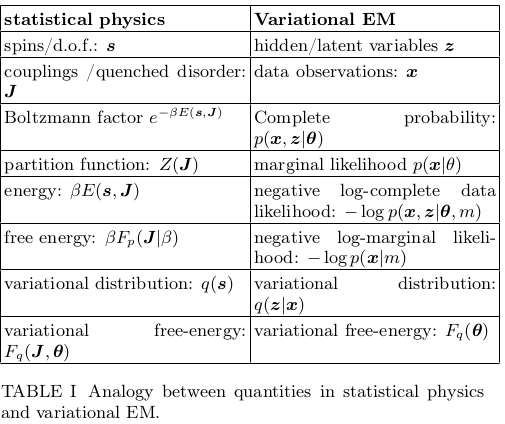
\includegraphics[width=0.7\linewidth]{gfx/AnalogyEMstatphys}
	\caption{}
	\label{fig:analogyemstatphys}
\end{figure}









\section{Energy Based Models: Maximum Entropy (MaxEnt) Principle, Generative Models, and Boltmann Learning}
\label{sec:energy}
\subsection{Introduction - Why do we need another class of models}
Supervised learning models discussed in \ref{ch:supervised} are \emph{discriminative} - they are designed to perceive differences between groups or categories of data. Discriminative models form the core techniques of most supervised learning methods, but they have several limitations.
\begin{enumerate}
	\item They require labelled data.
	\item There are tasks that discriminative approaches simply cannot accomplish, such as drawing new examples from an unknown probability distribution. 
\end{enumerate}

	A model that can earn to represent and sample from a probability distribution is called \emph{generative}. \emph{Energy-based} generative models are able to deal with tasks discriminative models even fail to attempt in the first place. This section is concerned with introducing these models.

\subsection{An overview of energy-based generative models}
\label{subsec:energyOverview}
\subsubsection{The idea}
This overview will highlight the similarities and differences with the supervised learning methods encountered in earlier sections.\\
\begin{mybox}{Generative model idea}
	Generative models are a ML technique that allows to learn how to generate new examples similar to those found in a training dataset. The core idea of most generative models is to learn a parametric model for the probability distribution from which the data was drawn. One we have learned a model, we can generate new examples by sampling from the learned generative model. As in stat. phys., this sampling is often done using MCMC methods.
\end{mybox}
The added complexity of learning models directly from samples introduces many of the same fundamental tensions we encountered when discussing discriminative models. The ability to generate new examples requires models to be able to "generalize" beyond the examples they have been trained on, that is to generate new samples that are not samples of the training set. The models must be expressive enough to capture the complex correlations present in the underlying data distribution, but the amount of data we have is finite which can give rise to overfitting.
\subsubsection{Generative models in practice}
In practice, most generative models that are used in ML are flexible enough that, with a sufficient number of parameters, they can approximate any probability distribution. For this reason,there are three axes on which we can differentiate classes of generative models:
\begin{enumerate}
	\item First axis is how easy the model is to train - both in terms of computational time and the complexity of writing code for the algorithm.
	\item The second axis is how well the model generalizes from the training set to the test set.
	\item The third axis is which characteristics of the data distribution the model is capable of and focuses on capturing.
\end{enumerate}
All generative models must balance these competing requirements and generative models differ in the tradeoffs they choose.\\
\\
One of the fundamental reasons that energy-based models have been less widely-employed than their discriminative counterparts is that the training procedure for these models differs significantly from those for supervised NNs (\ref{sec:dnn},\ref{sec:cnn},\ref{sec:dnn2}). Though both employ GD \ref{sec:gd} based procedure for minimizing a cost function (one common choice for generative models is the negative log-likelihood function \ref{eq:bayesErrorFct}), energy-based models do not use backpropagation\ref{subsec:dnnBackpropagation} and automatic differentiation for computing gradients. Rather, one must turn to ideas inspired by MCMC based methods in physics and statistics that sometimes go under the name "\emph{Boltzmann learning}". As a result, training energy-based models requires additional tools that are not immediately available in packages such as PyTorch and TensorFlow.\\
The open-source package \emph{Paysage} that is built on top of PyTorch bridges this gap by providing the toolset for training energy-based models. Paysage makes it easy to quickly code and deploy energy-based models such as Restricted Boltzmann Machines (RBMs) and Stacked RBMs - a "deep" unsupervised model.\\
\\
	Finally, we note that generative models at their most basic level are complex parametrizations of the probability distribution the data is drawn from. For this reason, generative models can do much more than just generate new examples. They can be used to perform a multitude of other tasks that require sampling from a complex probability distribution including "de-noising", filling in missing data, and even discrimination. The versatility of generative models is one of the major appeals of these unsupervised learning methods.


\subsection{Maximum entropy models: the simplest energy-based generative models}
\label{subsec:energyMaxEnt}
MaxEnt models have no latent (or hidden) variables, making them ideal for introducing the key concepts and tools that underlie energy-based generative models.
\subsubsection{Derivation of the theory}
It is possible to rederive the Boltzmann distribution (and the idea of generalized ensembles) entirely from information theoretic arguments. The Boltzmann distribution can be viewed as resulting from a statistical inference procedure for learning probability distributions describing physical systems where one only has partial information about the system (usually the average energy).\\
The key quantity in MaxEnt models is the information theoretic, or Shannon, entropy \ref{eq:infoShannon}. The Boltzmann distribution follows from the Principle of Maximum Entropy.
\begin{mybox}{Principle of Maximum Entropy}
A physical system should be described by the probability distribution with the largest entropy subject to certain constrains (often provided by measuring the average value of conserved, extensive quantities such as energy, particle number,..). The principle uniquely specifies a procedure for parametrizing the functional form of the probability distribution. Once we have specified and learned this form we can, of course, generate new examples by sampling this distribution.
\end{mybox}
How does this work ?\\
Suppose that we have chosen a set of functions $\{f_i(\mx)\}$ whose average value we want to fix to some observed values $\expval{f_i}_{obs}$. The Principle of Maximum Entropy states that we should choose the distribution $p(\mx)$ with the largest uncertainty (i.e. the largest Shannon entropy $S_p$ \ref{eq:infoShannon}), subject to the constraints that the model averages match the observed averages
\be 
\expval{f_i}_{model} = \int \md \mx f_i(\mx) p(\mx) = \expval{f_i}_{obs}.
\ee 
We can formulate the Principle of Maximum Entropy as an optimization problem using the method of Lagrange multipliers by minimizing 
\begin{align*}
	\mL[p] &= -S_p + \sum_i \lambda_i \left(\expval{f_i}_{obs} - \int \md \mx f_i (\mx) p(\mx) \right)\\
	&+ \gamma \left(1- \int \md \mx p(\mx)\right)\\
	0&=\frac{\delta \mL}{\delta p} = (\log p(\mx) +1) - \sum_i \lambda_i f_i(\mx) -\gamma,
\end{align*}
where the first set of constraints enforce the requirement for the averages and the last constraint enforces the normalization that the trace over the probability distribution equals one. The differentiation leads to the general form of the maximum entropy distribution
\be 
p(\mx) = \frac{1}{Z} e^{\sum_i \lambda_i f_i(\mx)}
\ee 
where $Z(\lambda_i)= \int \md \mx e^{\sum_i \lambda_i f_i(\mx)}$ is the partition function. The maximum entropy distribution is clearly just the usual Boltzmann distribution with energy $E(\mx) = - \sum_i \lambda_i f_i(\mx)$. The values of the Lagrange multipliers are chosen to match the observed averages for the set of functions $\{f_i(\mx)\}$ whose average value is being fixed:
\bse 
\expval{f_i}_{model}=\int \md \mx p(\mx) f_i(\mx) = \frac{\partial \log Z}{\partial \lambda_i} = \expval{f_i}_{obs}.
\ese 
In other words, the parameters of the distribution can be chosen such that 
\bse 
\partial_{\lambda_i} \log Z= \expval{f_i}_{data}.
\ese 
\begin{mybox}{Comparison to stat. phys.}
	Our $\mx$ denotes the microscopic state of the system, i.e. the MaxEnt distribution is a probability distribution over microscopic states. However, in thermodynamics we only have access to average quantities. If we know only the average energy $\expval{E(\mx)}_{obs}$, the MaxEnt procedure tells us to maximize the entropy subjet to the average energy constraints, this yields
	\be 
	p(\mx) = \frac{1}{Z} e^{-\beta E(\mx)},
	\ee 
	where we identified $\lambda_1 = - \beta= -1/k_BT$. Now suppose we also constrain the particle number $\expval{N(x)}_{obs}$. Then we obtain the following MaxEnt distribution
	\be 
	p(\mx) = \frac{1}{Z} e^{-\beta (E(\mx) - \mu N(\mx))},
	\ee 
	where we identified $\lambda_1=-\beta, \lambda_2=\mu/\beta$. Since this is just the Boltzmann distribution, we can also relate the partition function in our MaxEnt model to the thermodynamic free-energy via $F=-\beta^{-1} \log Z$. The choice of which quantities to constrain is equivalent to working in different thermodynamic ensembles.
\end{mybox}
\subsubsection{From statistical mechanics to ML}
The MaxEnt idea also provides a general procedure for learning a generative model from data. They key difference between MaxEnt models in physics and ML is that in ML we have no direct access to observed values $\expval{f_i}_{obs}$. Instead, these averages must be directly estimated from data (samples). To denote this difference, we will call empirical averages calculated from data as $\expval{f_i}_{data}$. We can think of MaxEnt as a statistical inference procedure simply by replacing $\expval{f_i}_{obs}$ by $\expval{f_i}_{data}$ as above.\\
This subtle change has important implications for training MaxEnt models. 
\begin{enumerate}
\item First, since we do not know these averages exactly, but must estimate them from the data, our training procedures must be careful not to overfit to the observations (our samples might no be reflective of the true values of these statistics). 
\item Second, the averages of certain functions $f_i$ are easier to estimate from limited data than others. This is often an important consideration when formulating which MaxEnt model to fit to the data.
\item Finally, we note that unlike in physics where conservation laws often suggest the functions $f_i$ whose averages we hold fix, ML offers no comparable guide for how to choose the $f_i$ we care about.
\end{enumerate}
For these reasons, choosing the $\{f_i\}$ is often farm from straightforward.\footnote{Note that MaxEnt is closely related to Bayesian inference from a ML perspective.}

\subsubsection{Generalized Ising models from MaxEnt}
The form of a MaxEnt model is completely specified once we choose the averages $\{f_i\}$ we wish to constrain. One common choice often used in MaxEnt modeling is to constrain the first two moments of a distribution. When our random variables $\mx$ are continuous, the corresponding MaxEnt distribution is a multi-dimensional Gaussian. If the $\mx$ are binary (discrete), then the corresponding MaxEnt distribution is a generalized Ising (Potts) model with all-to-all couplings.\\
\\
Partition functions for maximum entorpy models are often intractable to compute. Therefore, it is helpful to consider two special cases where $\mx$ has different support (different kinds of data). 
\begin{enumerate}
	\item First, consider the case that the random variable $\mx \in \mR^n$ are real numbers. The partition function can be calculated analytically
	\bse 
	Z = \int \md x e^{\mathbf{a}^T \mathbf{x}+\half \mathbf{x}^TJ\mx}=\sqrt{(2\pi)^n \det J^{-1}} e^{- \half \mathbf{a}^T J^{-1} \mathbf{a}}.
	\ese
	The resulting probability density function is,
	\begin{align}
		\label{eq:energyCostfctMaxEntmodel}
		p(\mx) &= Z^{-1} e^{-E(\mx)} =\frac{1}{\sqrt{(2 \pi)^n \det J^{-1}} } e^{\half \mathbf{a}^T J^{-1} \mathbf{a}+ \mathbf{a}^T \mx+ \half \mx^T J \mx }\nonumber \\
		&=\frac{1}{\sqrt{(2 \pi)^n \det \Sigma} } e^{-\half (\mx -\mu)^T \Sigma^{-1} (\mx-\mu)},
	\end{align} 
where $\mu=-J^{-1} \mathbf{a}$ and $\Sigma = - J^{-1}$. This, of course, is the normalized, multi-dimensional Gaussian distribution.
\item Second, consider the case that the random variable $\mx$ is a binary with $x_i \in \{-1,+1\}$. The partition function can no longer be computed in a closed form. This model is known as the Ising model in physics and as Markov Random Field in ML. Calculating partition function for the Ising model is intractable. For this reason, the best we can do is estimate it using numerical techniques such MCMC methods \todo{reference} or approximate methods like variational MFT methods \ref{sec:varMFT}. 
\end{enumerate}
Finally we note that ML and physics notation for binary variables differ ($x_i \in  \{0,1\}$ rather than $x_i \in \{\pm 1\}$), which can lead to confusion translating between literature or programming packages in ML and physics problems.





\subsection{Cost functions for training energy-based models}
\label{subsec:energyCostfctHowTo}
The MaxEnt procedure gives us a way if parametrizing an energy-based generative model.\\
	For any energy-based generative model, the energy function $E(\mx,\{\theta_i\} )$ depends on some parameters $\theta_i$ - couplings in the language of stat. phys.- that must be inferred directly from the data. For example, for the MaxEnt models the $\{\theta_i\}$ are just Lagrange multipliers $\{\lambda_i\}$. 
\begin{mybox}{Training procedure.}
The goal of the training procedure is to use the available training data to fit these parameters.\\
	Like in many other ML techniques, we will fit these couplings by minimizing a cost function using SGD \ref{subsubsec:gdSGD}. Such a procedure naturally separates into two parts: choosing an appropriate cost function, an calculating the gradient of the cost function with respect to the model parameters.
\end{mybox}
\begin{mybox}{Defining a cost function}
	 Formulating a cost function for generative models is a little bit trickier than for supervised, discriminative models. The objective of discriminative models is straightforward - predict the label from the features. However, what we mean by a "good" generative model is much harder to define using a cost function. We would like the model to generate examples similar to those we find in the training dataset. However, we would also like the model to generalize - we do not want the model to reproduce "spurious details" that are particular to the training dataset. Unlike for discriminative models, there is no straightforward idea like cross-validation on the data labels that neatly addresses this issue. For this reason, formulating cost functions for generative models is subtle and represent an important and interesting open are of research.
\end{mybox}
Calculating the gradients of energy-based models also turns out to be different than for discriminative models, such as DNNs. Rather than relying on automatic differentiation techniques and backpropagation, calculating the gradient requires drawing on intuitions from MCMC-baed methods.\\
\\
What follows is an in-depth discussion of \emph{Boltzmann learning} for energy-based generative models, focussing on MaxEnt models. We put the emphasis on training procedures that generalize to more complicated generative models with latent variables such as RBMs.






\subsubsection{Maximum likelihood}
By far the most common approach used for training a generative model is to maximize the log-likelihood of the training data set. Recall, that the log-likelihood characterizes the log-probability of generating the observed data using our generative model. By choosing the negative log-likelihood as the cost function, the learning procedure tries to find parameters that maximize the probability of the data.\\
In what follows, we employ a general notation that is applicable to all energy-based models, not just the MaxEnt models \ref{subsec:energyMaxEnt}. The reason for this is that much of this discussion does not rely on the specific form of the energy function but only on the fact that our generative model takes a Boltzmann form. We denote the generative model by the probability distribution $p_{\theta}(\mx)$ and its corresponding partition function by $\log Z(\{\theta_i\})$. In MLE, the parameters of the model are fit by maximizing the log-likelihood
\be 
\label{eq:energyCostfctLogLikely}
\mL(\{\theta_i\}) = \expval{\log(p_{\theta}(\mx))}_{data}=-\expval{E(\mx;\{\theta_i\})}_{data} - \log Z(\{\theta_i\}),
\ee 
where we made use of 
\begin{enumerate}
	\item Our generative distribution is of the Boltzmann form, and
	\item the partition function does not depend on the data
	\bse 
	\expval{Z}_{data}=Z.
	\ese 
\end{enumerate}


\subsubsection{Regularization}
\label{subsubsec:energyCostfctRegularization}
Just as for discriminative models like linear and logistic regression, it is common to supplement the log-likelihood with additional regularization terms (cf. \ref{subsec:lregRegularization}). Instead of minimizing the negative log-likelihood, one minimizes a cost function of the form
\be 
-\mL(\{\theta_i\}) +E_{reg}(\{\theta_i\}),
\ee 
where $E_{reg}(\{\theta_i\})$ is an additional regularization term that prevents overfitting. From a Bayesian perspective, this new term can be viewed as encoding a (negative) log-prior on model parameters and performing a maximum-a-posteriori (MAP) estimate instead of a MLE.
\begin{mybox}{Regularization energy based models}
	A common choice for the regularization function are the sums of the $L_1$ or $L_2$ norms of the parameters
	\be 
	\label{eq:energyCostfctRegularizationFct}
	E_{reg}(\{\theta_i\}) = \Lambda \sum_i \abs{\theta_i}^\alpha ,\quad \alpha=1,2
	\ee 
	with $\Lambda$ controlling the regularization strength. A large $\Lambda$ will force many parameters to be close to or exactly zero, $\Lambda=0$ is MLE. Just as in regression, an $L_1$ penalty enforces sparsity, with many of the $\theta_i$ set to zero, and $L_2$ regularization shrinks the size of the parameters towards zero.
\end{mybox}
One challenge of generative models is that is is often difficult to choose the regularization strength $\Lambda$. Recall that, for linear \ref{sec:linearRegression} and logistic regression \ref{sec:logisticRegression}, $\Lambda$ is chosen to maximize the out-of-sample performance on a validation dataset (i.e. cross-validation). However, for generative models our data are usually unlabelled. Therefore, choosing a regularization strength is more subtle and there exists no universal procedure for choosing $\Lambda$. One common strategy is to divide the data into a training set and a validation set and monitor a summary statistic such as the log-likelihood, energy distance, or variational free-energy \ref{subsubsec:varMFTEMphys} of the generative model on the training and validation sets. If the gap between the training and validation datasets starts growing, one is probably overfitting the model even if the log-likelihood of the training dataset is still increasing. This also give a procedure for "early stopping".\\
In practice, when using such regularizers it is important to try many different values of $\Lambda$ and then try to use a proxy statistic for overfitting to evaluate the optimal choice of $\Lambda$.



\subsection{Computing gradients}
\label{subsec:energyGradients}
We still need to specify a procedure for minimizing the cost function. SGD \ref{subsubsec:gdSGD} is normally employed, but how do you actually compute the gradients ?\\
Define operators conjugate to the parameters $\theta_i$
\bse 
\mO_i(\mx) = \frac{\partial E(\mx;\theta_i)}{\partial \theta_i},
\ese 
which implies, as $Z$ is the cumulant generating function for the Boltzmann distribution, that
\bse 
\expval{\mO_i(\mx)}_{model}= \tr_{\mx} p_{\theta}(\mx) \mO_i(\mx) = -\frac{\partial \log Z(\{\theta_i\})}{\partial \theta_i}.
\ese 
\begin{mybox}{MLE}
Then, \ref{eq:energyCostfctLogLikely} becomes
\begin{align}
	\label{eq:energyGradientsMLE}
	-\frac{\partial \mL(\{\theta_i\})}{\partial \theta_i} &= \langle \frac{\partial E(\mx;\theta_i)}{\partial \theta_i}\rangle_{data} +\frac{\partial \log Z(\{\theta_i\})}{\partial \theta_i} \nonumber \\
	&=\expval{\mO_i(\mx)}_{data} - \expval{\mO_i(\mx)}_{model}.
\end{align}
The gradient of the log-likelihood w.r.t. a model parameter \ref{eq:energyGradientsMLE} is a difference of moments - one calculated directly from the data and one calculated from our model using the current model parameters. The data-dependent term is known as the \emph{positive phase} of the gradient and the model-dependent term is known as the \emph{negative phase} of the gradient. This derivation also gives an intuitive explanation for likelihood-based training procedures. The gradient acts on the model to lower the energy of configurations that are near observed data points while raising the energy of configurations that are far from observed data points. Finally, we note that all information about the data only enters the training procedure through the expectations $\expval{\mO_i(\mx)}_{data}$ and our generative model is blind to information beyond what is contained in these expressions. 
\end{mybox}
\subsubsection{How does one actually compute the gradient then ?}
To use SGD, we must still calculate the expectation values in \ref{eq:energyGradientsMLE}. The positive phase of the gradient can be easily calculated using samples from the training dataset. The negative phase, however, is generally much more difficult to compute because analytically calculating the partition function is intractable for most interesting models.
\begin{definition}
	There are exceptional cases in which we can calculate the expectation values analytically. When this happens, the generative model is said to have a \emph{Tractable Likelihood}. One example of a generative model with a Tractable Likelihood is the Gaussian MaxEnt model for real valued data \ref{eq:energyCostfctMaxEntmodel}.
\end{definition}
Returning to the generic case where most energy-based model have \emph{intractable likelihoods}, we must estimate expectation values numerically. One way to do this is draw samples $\mathcal{S}_{model} =\{\mx^\prime_i\}$ from the model $p_{\theta}(\mx)$ and evaluate arbitrary expectation values using these samples:
\be 
\expval{f(\mx)}_{model} = \int \md \mx p_\theta(\mx) f(\mx) \approx \sum_{\mx^\prime_i\in\mathcal{S}_{model}} f(\mx^\prime_i).
\ee 
The samples from the model $\mx^\prime_i\in\mathcal{S}_{model}$ are often referred to as \emph{fantasy particles} in the ML literature and can be generated using simple MCMC algorithms such as Metropolis-Hasting.\\
\\
Finally, we note that once we have the fantasy particles from the model, we can also easily calculate the gradient of any expectation value $\expval{f(\mx)}_{model}$ using what is commonly called the "log-derivative trick" in ML
\begin{align*}
	\frac{\partial}{\partial \theta_i} \expval{f(\mx)}_{model} &= \int \md \mx \frac{\partial p_\theta(\mx)}{\partial \theta_i} f(\mx) \\
	&= \langle \frac{\partial \log p_\theta(\mx)}{\partial \theta_i} f(\mx)\rangle _{model} \\
&= \expval{\mO_i(\mx) f(\mx)}_{model} \approx \sum_{\mx^\prime_j\in\mathcal{S}_{model}} \mO_i(\mx_j) f(\mx^\prime_j).
\end{align*}




\subsection{Summary of the training procedure}
\label{subsec:energyTrainingProcedure}
We now summarize the discussion above and present a general procedure for training an energy-based model using SGD on the cost function.
\begin{mybox}{Training Procedure - Recipe}
	Our goal is to fit the parameters of a model $p_{\lambda}(\{\theta_i\}) = Z^{-1} e^{-E(\mx,\{\theta_i\})}$. Training the model involves the following steps:
		\begin{enumerate}
			\item Read a minibatch of data, $\{\mx\}$.
			\item Generate fantasy particles $\{\mx^\prime\} \sim p_\lambda$ using an MCMC algorithm (e.g., Metropolis-Hastings).
			\item Compute the gradient of log-likelihood using these samples and \ref{eq:energyGradientsMLE}, where the averages are taken over the minibatch of data nad the fantasy particles from the model, respectively.
			\item Use the gradient as input to one of the gradient based optimizers from \ref{sec:gd}.
		\end{enumerate}
\end{mybox}
\subsubsection{Practical tips}
In practice, it is helpful to supplement this pasigc proecure with some tricks that help training. As with discriminative NNs, it is important to initialize the parameters properly and print summary statistics during the training procedure on the traing and validation sets to prevent overfitting. This is more discussed in \ref{subsubsec:deepGenerativeTrainingPractical}\todo{Cheap tricks, to compile and reference !}.











\section{Deep Generative Models: Hidden Variables and Restricted Boltzmann Machines (RBMs)}
\label{sec:deepGenerative}
Here, we extend the discussion in \ref{sec:energy} to energy-based models that include latent or hidden variables.\\
Including latent variables in generative models greatly enhances their expressive power allowing the model to represent sophisticated correlations between visible veatures without sacrificing trainability.

\subsection{Why hidden (latent) variables ?}
\label{subsec:deepGenerativeWhy}
\subsubsection{Idea}
Latent or hidden variables are a powerful yet elegant way to encode sophisticated correlations between observable features.

\begin{mybox}{Quintessence - physics perspective}
	The underlying reason for this is that marginalizing over a subset of variables -"integrating out" degrees of freedom in the language of physics - induces complex correlations is a familiar component of many physical theories. For example when considering free electrons living on a lattice, integrating out phonons gives rise to higher-order electron-electron interactions (e.g. superconducting or magnetic correlations). More generally, in the Wilsonian renormalization group paradigm, all effective field theories can be though of as arising form integrating out high-energy degrees of freedom.
\end{mybox}
Generative models with latent variables run this logic in reverse.
\begin{mybox}{Quintessence - generative models perspective}
	Encode complex interactions between visible variables by introducing additional, hidden variables that interact with visible degrees of freedom in a simple manner, yet still reproduce the complex correlations between visible degrees in the data once marginalized over (integrated out). This allows us to encode interactions between the visible variables using simpler interactions at the cost of introducing new latent variables/degrees of freedom.
\end{mybox}
This trick is also widely exploited in physics (e.g. in the Hubbard-Stratonovich transformation or the introduction of ghost fields in gauge theory).

\subsubsection{For example - the Ising model}
\label{subsubsec:deepGenerativeHopfield}
To make these ideas more concrete, let us revisit the pairwise Ising model, which is described by a Boltzmann distribution $p(\mathbf{v}) = e^{E(\mathbf{v})}/Z$ with energy 
\bse 
E(\mathbf{v}) = - \sum_i a_i v_i - \half \sum_{ij} v_i J_{ij} v_j,
\ese 
where $J_{ij}$ is a symmetric coupling matrix that encodes the pairwise constraints and $a_i$ enforce the single-variable constraint.\\
Our goal is to replace the complicated interactions between the visible variables $v_i$ encoded by $J_{ij}$, by interactions with a new set of latent variables $h_\mu$. In order to do this, it is helpful to rewrite the coupling matrix in a slightly different form. Using SVD, we can always express the coupling matrix in the form $J_{ij} = \sum_{\mu=1}^N W_{i \mu} W_{j\mu}$, where $\{W_{i\mu}\}$ are appropriately normalized singular vectors.
\begin{mybox}{Hopfield model}
	 In terms of $W_{i\mu}$, the energy takes the form
\be 
\label{eq:deepGenerativeHopfield}
E_{Hop}(\mathbf{v}) = -\sum_i a_i v_i - \half \sum_{ij \mu} v_i W_{i \mu} W_{ j\mu} v_j.
\ee 
We note that in the special case when both $v_i \in \{-1,+1\}$ and $W_{i\mu} \in \{-1,+1\}$ are binary variables, a model with this form of the energy functions is known as the \emph{Hopfield model}.
Note that here we will refer to all energy functions of the form\ref{eq:deepGenerativeHopfield} as (generalized) Hopfield models, even for the case when the $W_{i\mu}$ are continuous variables.
\end{mybox}
We now "decouple" the visible variables $v_i$ by introducing a set of normally, distributed continuous latent variables $h_\mu$ such that we can rewrite the Boltzmann distribution for the generalized Hopfield model as
\begin{align*}
	p(\mathbf{v}) &= \frac{e^{\sum_i a_i v_i+\half \sum_{ij\mu} v_i W_{i\mu} W_{j\mu} v_j} }{Z}\\
		&= \frac{e^{\sum_i a_i v_i} \prod_\mu \int \md h_\mu e^{-\half \sum_\mu h^2_\mu-\sum_i v_i W_{i\mu} h_\mu} }{Z} \\
		&\equiv \frac{\int \md \mathbf{h}e^{-E(\mathbf{h,v}) }}{Z},
\end{align*}
where $E(\mathbf{v,h})$ is a joint energy functional of both the latent and visible variables of the form
\be 
E(\mathbf{v,h}) = - \sum_i a_i v_i + \half \sum_\mu h^2_\mu - \sum_{i\mu} v_i W_{i\mu} h_\mu. 
\ee 
We can also use the energy function $E(\mathbf{v,h})$ to define a new energy-based model $p(\mathbf{v,h})$ on both the latent and visible variables
\be 
p(\mathbf{v,h}) = \frac{e^{-E(\mathbf{v,h}) }}{Z^\prime}.
\ee 
Marginalizing over latent variables of course gives us back the generalized Hopfield model
\be 
p(\mathbf{v}) =\int \md \mathbf{h}p(\mathbf{v,h}) = \frac{e^{-E_{Hop}(\mathbf{v})}}{Z}.
\ee 
Notice that $E(\mathbf{v,h})$ contains no direct interactions between visile degrees of freedom (or between hidden degrees of freedom). Instead, the complex correlations between the $v_i$ are encoded in the interaction between the visible $v_i$ and latent variables $h_\mu$. It turns out that the model presented here is a special case of a more general class of powerful energy-based models called Restricted Boltzmann Machines (RBMs).


\subsection{Restricted Boltzmann Machines (RBMs)}
\label{sec:deepGenerativeRBM}


\begin{figure}[h!]
	\centering
	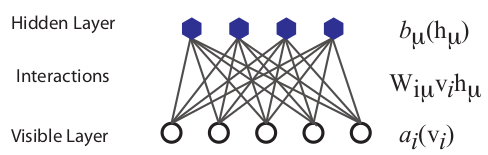
\includegraphics[width=0.5\linewidth]{gfx/RBM}
	\caption{\itshape A RBM consists of visible units $v_i$ and hidden units $h_\mu$ that interact with each other through interactions of the form $W_{i\mu}v_ih_\mu$. Importantly, there are no interactions between visible units themselves or hidden units themselves.}
	\label{fig:RBM}
\end{figure}

\begin{mybox}{RBM}
	A RBM is an energy-based model with both visible and hidden units where the visible and hidden units interact with each other but do not interact among themselves, compare figure \ref{fig:RBM}. The energy function of an RBM takes the general functional form
	\be 
	\label{eq:deepGenerativeRBMenergy}
	E(\mathbf{v,h}) = - \sum_i a_i (v_i) -\sum_\mu b_\mu (h_\mu) - \sum_{i\mu} W_{i\mu} v_i h_\mu,
	\ee 
	where $a_i(\cdot)$ and $b_\mu(\cdot)$ are functions that we are free to choose. The most common choice is:
		\bse 
a_i(v_i) = \Bigg\{
\begin{array}{ll}
	a_i v_i& \text{if $v_i\in \{0,1\}$ is binary}\\
	\frac{v^2_i}{2 \sigma^2_i}, & \text{if $v_i\in \mR$ is continuous}.
\end{array}
\ese 
		and,
		\bse 
		b_\mu(h_\mu) =\Bigg\{ \begin{array}{ll}
			b_\mu h_\mu & \text{if $h_\mu \in \{0,1\}$ is binary}\\
			\frac{h^2_\mu}{2 \sigma^2_\mu}, & \text{if $h_\mu\in \mR$ is continuous}.
	\end{array}
	\ese 
	For this choice of $a_i,b_\mu$, layers consisting of discrete binary units are often called \emph{Bernoulli layers}, and layers consisting of continuous variables are often called Gaussian layers.
\end{mybox}
The different possible combinations are the following.\\
 \begin{tabular}{|l|ll|}
	       Name &Visible Layer $a_i(v_i)$ & Hidden Layer $b_\mu(h_\mu)$ \\
	\toprule
"RBM" & Bernoulli & Bernoulli\\
Multi-dimensional Gaussian & Gaussian &Gaussian \\
Generalized Hopfield model& Bernoulli &Gaussian \\
Gaussian Bernoulli RBM & Gaussian &Bernoulli\\
	\bottomrule
\end{tabular}
\vspace{0.1cm}
Specifying a generative model with this bipartite interaction structure has two major advantages:
\begin{enumerate}
\item It enables capturing both pairwise \emph{and higher-order} correlations between the visible units and 
\item it makes it easier to sample from the model using an MCMC method known as block Gibbs sampling, which in turn makes the model easier to train.
\end{enumerate}

\subsubsection{Content of an RBM}
We want to understand the kind of correlations that can be captured using an RMB.\\
One can derive that the marginal energy includes all order of interactions between the visible units, with the $n$-th order cumulants of the distribution of hidden units $q_\mu(h_\mu) = e^{b_\mu(h_\mu)}/Z$ weighting the $n$-th order interactions between the visible units.\\
This exemplifies the incredible representational power of RBMs with a Bernoulli hidden layer. Each hidden unit can encode interactions of arbitrarily high order. By combining many different hidden units, we can encode very complex interactions at all orders. Moreover, we can learn which order of correlations/interactions are important directly from the data instead of having to specify them ahead of time as we did in the MaxEnt models \ref{subsec:energyMaxEnt}. This highlights the power of generative models with even the simplest interactions between visible and latent variables to encode, learn, and represent complex correlations present in the data.



\subsection{Training RBMs}
\label{subsec:deepGenerativeTraining}
RBMs are a special class of energy-based generative models, which can be trained using the MLE procedure described in detail in \ref{subsec:energyGradients},\ref{subsec:energyTrainingProcedure}. The gradient (SGD) can be calculated using \ref{eq:energyGradientsMLE}. As before calculating the negative phase of the gradient (i.e. the expectation value w.r.t. to the model) requires that we draw samples from the model. The bipartite form of the interactions in RBMs were specifically chosen with this in mind.

\subsubsection{Gibbs sampling and contrastive divergence (CD)}
\label{sububsec:deepGenerativeTrainingGibbsCD}
The bipartite interaction structure of an RBM makes it possible to calculate expectation values using a MCMC method known as Gibbs sampling. The key reason for this is that since there are no auto-interactions in the layers, the visible and hidden units of an RBM are conditionally independent:
\begin{align}
	\label{eq:deepGenerativeTrainingGibbsCDdistributions}
	p(\mathbf{v} |\mathbf{h}) &= \prod_i p(v_i|\mh),\; p(\mh|\mv) = \prod_\mu p(h_\mu|\mv) \nonumber \\
	p(v_i|\mh) &=\sigma(a_i +\sum_\mu W_{i\mu} h_\mu) \\
	p(h_\mu =1 |\mv) &= \sigma(b_\mu + \sum_i W_{i\mu} v_i)\nonumber,
\end{align}
and where $\sigma(z)=1/(1+e^{-z})$ is the sigmoid function.\\
\begin{mybox}{Procedure}
	Using these expressions it is easy to compute expectation values w.r.t. the data. The input to GD is a minibatch of observed data. For each sample in the minibatch, we simply clamp the visible units to the observed values and apply \ref{eq:deepGenerativeTrainingGibbsCDdistributions} using the probability for the hidden variables. We then average over all samples in the minibatch to calculate expectation values w.r.t. the data. To calculate expectation values w.r.t. the model, we use (block) Gibbs sampling. The idea behind (block) Gibbs sampling is to iteratively sample from the conditional distribution $\mh_{t+1} \sim p(\mh |\mv_t)$ and $\mv_{t+1} \sim p(\mv|\mh_{t+1})$. Since the units are conditionally independent, each step of this iteration can be performed by simply drawing random numbers. The samples are guaranteed to converge to the equilibrium distribution of the model in the limit that $t\rightarrow$. At the end of the Gibbs sampling procedure, one ends up with a minibatch of samples (fantasy particles).
\end{mybox}
To create a guaranteed independent sample, one resorts to using an approximate Gibbs sampling technique called \emph{Contrastive Divergence}(CD). In CD-$n$, we just perform $n$ interations of (block) Gibbs sampling, with $n$ often taken to be as small as $1$, it has proven to work reasonably well. Furthermore, to introduce stochasticity into the drawn dataset one uses a variant called Persistent CD (PCD). In PCD, rather than restarting the Gibbs sampler from the data at each GD step, we start the Gibbs sampling at the fantasy particles in the last GD step. Since parameters change slowly compared to the Gibbs sampling, samples that are high probability at one step of the SGD are also likely to be high probability at the next step. This ensures that PCD does not introduce large errors in the estimation of the gradients. The advantage of using fantasy particles to initialize the Gibbs sampler is to allow PCD to explore parts of the feature space that are much further from the training dataset than one could reach with ordinary CD, thus creating a randomized and independent minibatch via stochasticity.

\subsubsection{Practical Considerations}
\label{subsubsec:deepGenerativeTrainingPractical}
Important tricks in the application are the following.
\begin{enumerate}
	\item \emph{Initialization}.\\
	The model must be initialized. Hinton suggests taking the weights $W_{i\mu}$ from a Gaussian with mean zero and standard deviation $\sigma=0.01$. An alternative initialization scheme proposed by Glorot and Bengio instead chooses the standard deviation to scale with the size of the layers: $\sigma = 2/\sqrt{N_v+N_h}$ where $N_v$ and $N_h$ are number of visible and hidden units respectively. The bias of the hidden units is initialized to zero while the bias of the visible units is typically taken to be inversely proportional to the mean activation, $a_i=\expval{v_i}^{-1}_{data}$.
	\item \emph{Regularization}.\\
	One can of course use an $L_1$ or $L_2$ penalty, typically only on the weight parameters, not the biases. Alternatively, Droput has been shown to decrease overfitting when training with CD and PCD, which results in more interpretable learned features.
	\item  \emph{Learning rates}.\\
	Typically, it is helpful to reduce the learning rate in later stages of training.
	\item \emph{Updates for CD and PCD}.\\
	There are several computational tricks one can use for speeding up the alternating updates in CD and PCD, linked in Hinton $2012$.
\end{enumerate}




\subsection{Deep Boltzmann Machine}
\label{subsec:deepGenerativeDBM}
\subsubsection{The idea}
Unlike RBMs, DBMs possess multiple hidden layers and were the first models rebranded as "deep learning".
Basically, you stack RBMs, the idea is the following.\\
First of all we note the quintessential properties of RBMs again and their shortcomings.\\
An RBM is composed of two layers of neurons that are connected via an undirected graph \ref{fig:RBM}. As a result, it is possible to perform sampling $\mathbf{v}\sim p(\mathbf{v|h})$ and inference $\mh \sim p(\mh|\mv)$ with the same model. As with the Hopfield model \ref{eq:deepGenerativeHopfield}, we can view each of the hidden units as representative of a pattern, or feature, that could be present in the data.\footnote{In general, one should instead think of activity patterns of hidden units representing features in the data.} The inference step involves assigning a probability to each of these features that expresses the degree to which each featue is present in a given data sample. In an RBM, hidden units do not influence each other during the inference step, i.e. hidden unit are conditionally independent given the visible units. How can we create connections between the hidden units ? This is essentially what a DBM boils down to.
\begin{mybox}{DBM idea}
	For a DBM, you stack multiple RBMs together to generate intra-layer interactions. How do we do this ?\\
	With the Hopfield model, we saw that pairwise lienar connections between neurons can be mediated through another layer. Therefore, a simple way to allow for effective connections between the hidden units is to add another layer of hidden units. Rather than just having two layers, one visible and one hidden, we can add additional layers of latent variables to account for the correlations between hidden units. Ideally, as one adds more and more layers, one might hope that the correlations between hidden variables become smaller and smaller deeper into the network. This basic logic is reminiscent of renormalization procedures that seek to decorrelate layers at each step.
\end{mybox}
The price of adding additional layers is that the models become harder to train.
\subsubsection{Training a DBM}
\label{subsubsec:deepGenerativeDBMTraining}
Training DBMs is more subtle than RBMs due to the difficulty of propagating information from visible to hidden units. Some of these problems can be alleviated via a layer-wise procedure.\\
Rather than attempting to train the whole DBM at once, we can think of the DB; as a stack of RBMs, compare figure \ref{fig:dbm}.
\begin{mybox}{Training procedure}
	One first trains the bottom two layers of the DBM - treating it as if it is a stand-alone RBM. Once this bottom RBM is trained, we can generate "samples" from the hidden layer and use these samples as an input to the next RBM (consisting of the first and second hidden layer - purple hexagons and green squares in Fig. \ref{fig:dbm}). This procedure can then be repeated to pretrain all layers of the DBM.
\end{mybox}
This pretraining initializes the weights so that SGD can be used effectively when the network is trained in a supervised fashion. In particular, the pretraining helps the gradients to stay well-behaved rather than vanish or blow up (cf. \ref{subsubsec:dnnBackpropagationProblems}).\\
It is worth noting that once pretrained, we can use the usual Boltzmann learning rules in \ref{eq:energyGradientsMLE} to fine-tune the weights and improve the performance of the DBM. As we demonstrate in the following, the Paysage packaged can be used to both construct and train DBMs using such a pretraining procedure.





\begin{figure}[h!]
	\centering
	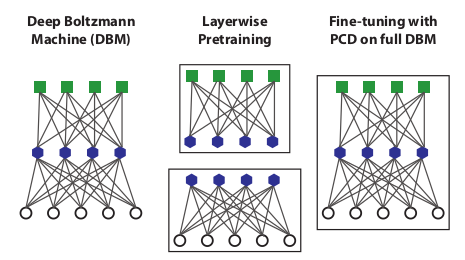
\includegraphics[width=0.7\linewidth]{gfx/DBM}
	\caption{\itshape Deep Boltzmann Machine contain multiple hidden
		layers. To train deep networks, first we perform layerwise
		training where each two layers are treated as a RBM. This
		can be followed by fine-tuning using gradient descent and per-
		sistent contrastive divergence (PCD).}
	\label{fig:dbm}
\end{figure}








































 